% article.tex - Main article content

\begin{abstract}
Open data sharing is increasingly mandated by research funders, journals, and institutions, yet large-scale compliance measurement remains challenging. We analyzed approximately \num{326000} open access biomedical research articles published between January 2024 and December 2025 using PDF-based text extraction (MinerU) combined with algorithmic detection of data sharing statements (oddpub v7.2.3), enriched with funder, journal, and institutional metadata from OpenAlex. We found an overall open data rate of 8.7\%, rising to 16.6\% among funded articles. Rates varied more than tenfold across the research ecosystem: top funders achieved 30--53\% (e.g., Uppsala UPPMAX 52.7\%, Science for Life Laboratory 49.1\%, European Molecular Biology Laboratory 46.7\%), while top journals reached observed rates of 70--86\%, with corrected estimates as high as 92.9\% (Nature Genetics) after adjusting for XML-only coverage limitations. PDF-based detection identified approximately 52\% more data sharing statements than XML-based methods on the same articles. These findings demonstrate that funder and journal policies substantially influence open data practices, and that current overall sharing rates remain far below universal compliance. An interactive dashboard at \url{https://www.opensciencemetrics.org} enables stakeholders to explore and benchmark these results.
\end{abstract}


\section{Introduction}

Data sharing has become a shared priority of biomedical research funders worldwide, anchored by policies from the NIH \cite{National-Institutes-of-Health2020-ed}, the European Commission \cite{European-Commission2021-fu}, UK Research and Innovation \cite{UK-Research-and-Innovation2016-gm}, the Wellcome Trust \cite{Wellcome-Trust2017-rs}, the Deutsche Forschungsgemeinschaft \cite{Deutsche-Forschungsgemeinschaft2019-ef}, the Swiss National Science Foundation \cite{Swiss-National-Science-Foundation2017-el}, the Agence Nationale de la Recherche \cite{Agence-Nationale-de-la-Recherche2019-mo}, and the US National Science Foundation \cite{National-Science-Foundation2023-ij}, as well as multilateral frameworks including the FAIR Data Principles \cite{Wilkinson2016-ap} and the UNESCO Recommendation on Open Science \cite{UNESCO2021-vq}.

The open science movement has placed data sharing at the center of efforts to improve the transparency and reproducibility of research. The FAIR principles---that research data should be Findable, Accessible, Interoperable, and Reusable---have become a widely endorsed framework for scientific data stewardship~\cite{Wilkinson2016-ap}. Meanwhile, surveys consistently reveal that a majority of researchers have encountered difficulties reproducing published results, underscoring the practical importance of access to underlying data~\cite{Baker2016-yj}. Studies have also demonstrated that publications linking to shared datasets receive more citations, creating incentive structures that complement institutional mandates~\cite{Colavizza2020-jf}.

In response, major research funders have adopted data sharing requirements of varying specificity and enforcement. The United States National Institutes of Health (NIH) implemented its Data Management and Sharing Policy in January 2023, requiring all NIH-funded researchers to submit data management plans and share scientific data~\cite{NIH2023dms}. The Wellcome Trust has required data sharing for all funded research since 2017~\cite{Wellcome-Trust2017-rs}, and the European Research Council has similarly mandated open access to research data generated by ERC-funded projects~\cite{European-Research-Council2017-mp}. These policies differ in stringency, scope, and enforcement mechanisms, creating a natural experiment in the effectiveness of policy design.

Journals have also emerged as influential gatekeepers of data sharing. Many high-impact journals now require data availability statements or deposit of data in public repositories as a condition of publication. Nature Research journals, Cell Press titles, and PLOS journals have progressively strengthened their data sharing policies over the past decade. However, the relationship between policy existence and actual compliance is not straightforward: previous work has shown that data availability statements do not always correspond to genuinely accessible data~\cite{Serghiou2021-pl}.

Measuring data sharing at scale is essential for evaluating whether these policies achieve their intended effects. Without systematic measurement, funders cannot benchmark their grantees' compliance, journals cannot assess the impact of editorial policies, and institutions lack the data needed to support their researchers. Yet scalable measurement presents significant methodological challenges. Manual assessment of data sharing is labor-intensive and impractical for large corpora. Text-mining approaches, while scalable, have historically relied on XML-formatted full text available through PubMed Central (PMC), which covers only a subset of published articles and may miss data sharing statements present in PDF-formatted sections such as supplementary materials.

Previous large-scale assessments of research transparency have provided valuable baselines. Serghiou et al.\ analyzed biomedical articles using XML-based detection and documented the prevalence of multiple transparency indicators including data sharing~\cite{Serghiou2021-pl}. However, XML-based approaches are limited by their inability to capture text from PDF-only articles or sections not represented in the XML markup. This limitation is substantial: in our corpus, a large fraction of articles lack PDF-based text extraction, and the detection rate among XML-only articles is systematically lower.

We address these limitations using a PDF-first detection pipeline. Full-text PDFs are processed using MinerU~\cite{Wang2024mineru}, a machine learning-based document extraction tool, and the resulting text is analyzed by oddpub v7.2.3~\cite{Riedel2020-fk}, an algorithm that identifies open data and open code sharing statements through pattern matching. This combination captures data sharing statements that XML-based methods miss, including those in supplementary sections, figure captions, and formatted data availability statements. On articles with both PDF and XML coverage, our PDF-based pipeline detects approximately 52\% more open data statements than XML alone.

In this study, we present the largest cross-funder, cross-journal comparison of open data sharing rates in biomedicine to date. We analyze approximately \num{326000} open access research articles from PubMed Central published between January 2024 and December 2025, characterizing data sharing rates across 816 funders and \num{1389} journals. We apply journal-level correction factors derived from head-to-head PDF versus XML comparisons to account for differential coverage, and report both observed and estimated open data rates with 95\% confidence intervals. Our results reveal more than tenfold variation in data sharing rates across the research ecosystem, with clear signals that funder and journal policies are associated with substantially higher compliance.

All results are available through an interactive dashboard at \url{https://www.opensciencemetrics.org}, enabling funders, journal editors, institutional administrators, and researchers to explore the data across multiple dimensions.


\section{Methods}

\subsection{Data Collection}

We retrieved metadata for all open access research articles indexed in PubMed Central published between January 2024 and December 2025, yielding a corpus of approximately \num{326000} articles. Full-text PDFs were downloaded from the PMC Open Access subset where available. Article-level metadata---including journal of publication, funder information, and author institutional affiliations---was obtained from OpenAlex~\cite{Priem2022-wr}, an open bibliographic database that aggregates records from Crossref, PubMed, institutional repositories, and other sources.

\subsection{PDF Processing and Open Data Detection}

PDFs were processed using MinerU~\cite{Wang2024mineru}, a machine learning-based extraction tool optimized for scientific documents that preserves document structure including tables, figures, and supplementary sections. The extracted text was then analyzed using oddpub v7.2.3~\cite{Riedel2020-fk}, an algorithm that detects open data and open code sharing statements in scientific publications through pattern matching against a curated dictionary of data sharing phrases, repository names, and accession number formats. Each article was classified as containing (or not containing) an open data statement and an open code statement.

For articles without available PDFs, we used the PMC XML full text as the input to oddpub. This dual-source approach maximized corpus coverage while enabling head-to-head comparison of detection rates between the two extraction methods.

\subsection{Metadata Enrichment}

Funder names reported in OpenAlex were normalized using a curated alias mapping covering 816 funders to aggregate related entities. For example, individual NIH institutes (e.g., NIMH, NIAID, NCI) were aggregated under their parent organization where appropriate, with child institute article counts deduplicated to avoid double-counting. This mapping was adapted from the funder normalization table used in the Open Science Metrics pipeline. OpenAlex works counts were used to filter for established funders, excluding small or niche entities with fewer than \num{100000} aggregated works from the main figures while retaining them in supplementary rankings.

Journal names were taken directly from the OpenAlex \texttt{primary\_location.source.display\_name} field. Institutional affiliations were extracted from the \texttt{authorships} metadata in OpenAlex.

\subsection{Statistical Analysis}

Open data rates were calculated as the proportion of articles with detected sharing statements, expressed as percentages. For the funder analysis, the baseline comparison rate was 16.6\% (the open data rate across all articles with at least one identified funder). For the journal analysis, the baseline was 8.7\% (the overall rate across all articles in the corpus).

\subsubsection{Correction Factors for XML-Only Articles}

Because PDF-based text extraction detects more data sharing statements than XML-based extraction, articles with only XML coverage have systematically underestimated open data rates. We developed a correction procedure using the subset of articles with both PDF and XML text (the ``head-to-head'' subset). For each journal with sufficient head-to-head data, we computed the ``best'' detection rate as the proportion of articles where \emph{either} the PDF or XML extraction identified an open data statement. This best rate represents our estimate of the true open data rate for that journal, since it combines the complementary strengths of both extraction methods.

For articles with only XML coverage, we applied the journal-specific best detection rate as a correction factor. The corrected open data count for a given entity (funder or journal) was calculated as:
\begin{equation}
\hat{N}_{\text{OD}} = N_{\text{OD,PDF}} + \sum_{j} n_{j,\text{XML}} \times r_{j,\text{best}}
\end{equation}
where $N_{\text{OD,PDF}}$ is the observed open data count among PDF-covered articles, $n_{j,\text{XML}}$ is the number of XML-only articles in journal~$j$, and $r_{j,\text{best}}$ is the best detection rate for journal~$j$ from the head-to-head subset. For journals without sufficient head-to-head data, a global fallback rate was used. The corrected estimate was floored at the observed count to ensure that corrections never reduce an already-observed signal.

Confidence intervals were computed using the Wilson score method~\cite{Wilson1927} on the head-to-head proportions and propagated through the weighted correction. All confidence intervals reported are 95\% Wilson score intervals.

\subsubsection{Figure Inclusion Thresholds}

To focus figures on well-powered entities, we applied Weibull-derived survival thresholds to determine the minimum article count for inclusion. Funders required at least \num{2586} funded articles and \num{100000} aggregated OpenAlex works for the main figure; journals required at least \num{1832} articles. These thresholds were selected to retain entities above the inflection point of the Weibull survival distribution fitted to entity-level article counts, ensuring that displayed rates are based on sufficient sample sizes. All entities above the minimum analysis threshold (100 articles for funders) are included in the supplementary tables.


\section{Results}

\subsection{Overall Open Data Rates}

Across our corpus of approximately \num{326000} open access biomedical research articles published in 2024--2025, we detected open data sharing statements in 8.7\% of publications, establishing a baseline rate for recent biomedical literature. Among the subset of articles with at least one identified funder, the rate was 16.6\%, nearly double the overall baseline, suggesting that funding is itself associated with higher data sharing.

\subsection{Variation by Funder}

Open data rates varied substantially across the 816 funders analyzed (Table~\ref{tab:funders}, Figure~\ref{fig:funders}). The top-ranked funders achieved observed rates three to six times higher than the 16.6\% funded-article baseline.

\begin{figure}[htbp]
\centering
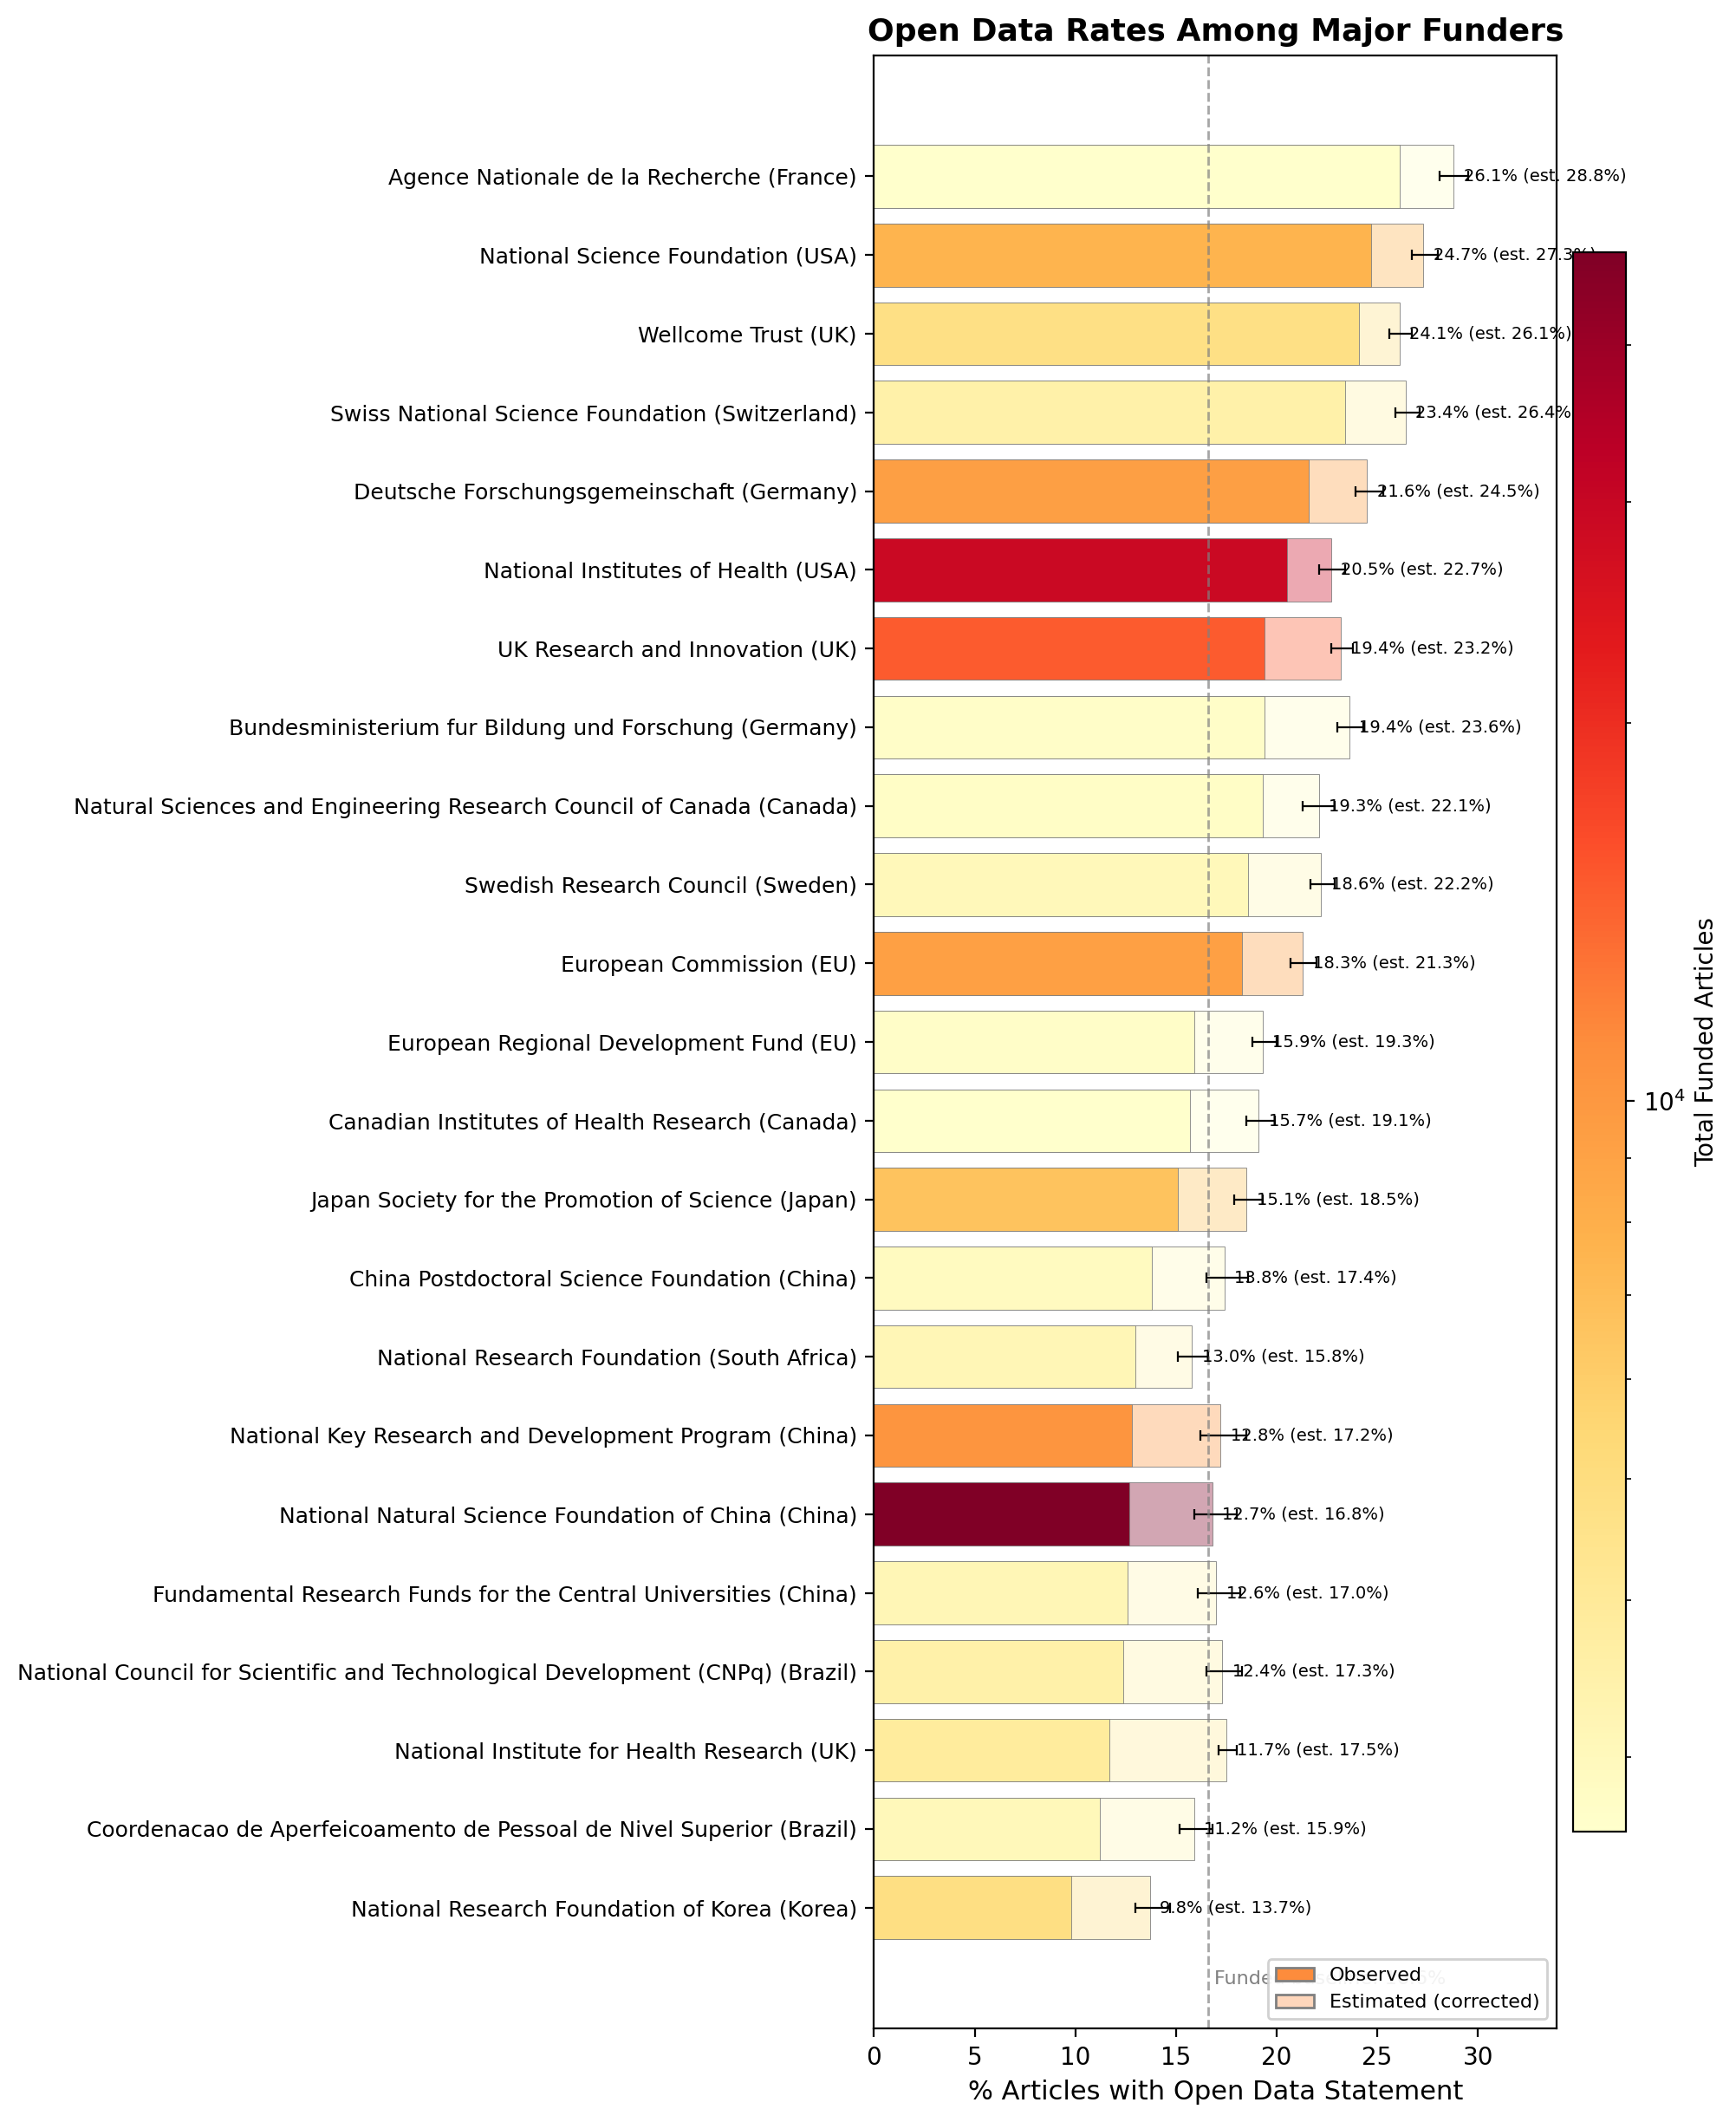
\includegraphics[width=\textwidth]{figures/funders_open_data_2024_2025.png}
\caption{Open data rates among major biomedical research funders (2024--2025 research articles). Bar length shows the observed open data rate (full opacity) and the estimated corrected rate (lighter shade) after applying journal-level PDF vs.\ XML correction factors. Error bars indicate 95\% Wilson score confidence intervals on the corrected estimate. Bar color encodes total funded article count on a log scale (yellow = fewer, red = more). Dashed line shows the funded-article baseline. Only funders exceeding both the Weibull-derived 3\% survival article-count threshold and 100{,}000 aggregated OpenAlex works are shown.}
\label{fig:funders}
\end{figure}

Swedish research organizations led the rankings: the Uppsala Multidisciplinary Center for Advanced Computational Science (UPPMAX) achieved the highest observed rate at 52.7\% (59 of 112 articles), followed by the Science for Life Laboratory (SciLifeLab) at 49.1\% (108 of 220 articles). Both organizations are closely affiliated with Sweden's national bioinformatics infrastructure, where data sharing is deeply embedded in research workflows.

European research organizations were prominently represented among the top performers. The European Molecular Biology Laboratory (EMBL) achieved 46.7\% (57 of 122 articles), the Francis Crick Institute 40.1\% (73 of 182), and the European Molecular Biology Organization (EMBO) 36.7\% (106 of 289). German funders including the Deutsches Krebsforschungszentrum (38.7\%), the Leibniz Association (33.8\%), and the Max Planck Society (30.6\%, 293 of 958 articles) all substantially exceeded the baseline. French funders including the Fondation ARC pour la Recherche sur le Cancer (37.9\%), the European Synchrotron Radiation Facility (37.8\%), and INRAE (35.7\%) showed a similar pattern.

Among United States funders, the Department of Energy's Biological and Environmental Research program achieved 40.6\% (108 of 266 articles) and the Argonne National Laboratory reached 43.6\% (68 of 156). The NIH Common Fund (35.6\%), the NSF Directorate for Biological Sciences (34.8\%, 288 of 828 articles), and the DOE Office of Science (31.3\%, 233 of 744) all demonstrated rates well above the funded-article baseline. Private philanthropies also performed strongly: the Howard Hughes Medical Institute achieved 34.9\% (261 of 748 articles) and the Burroughs Wellcome Fund 32.5\%.

Canadian funders including the Canadian Institute for Advanced Research (42.9\%) and Genome Canada (35.0\%) appeared in the top 20, as did the Swiss \'{E}cole Polytechnique F\'{e}d\'{e}rale de Lausanne (32.9\%) and ETH Z\"{u}rich (28.3\%).

\subsection{Variation by Journal}

Journal-level open data rates showed even greater variation than funder rates, spanning from below 5\% to above 90\% estimated (Table~\ref{tab:journals_2024_2025}, Figure~\ref{fig:journals}).

\begin{figure}[htbp]
\centering
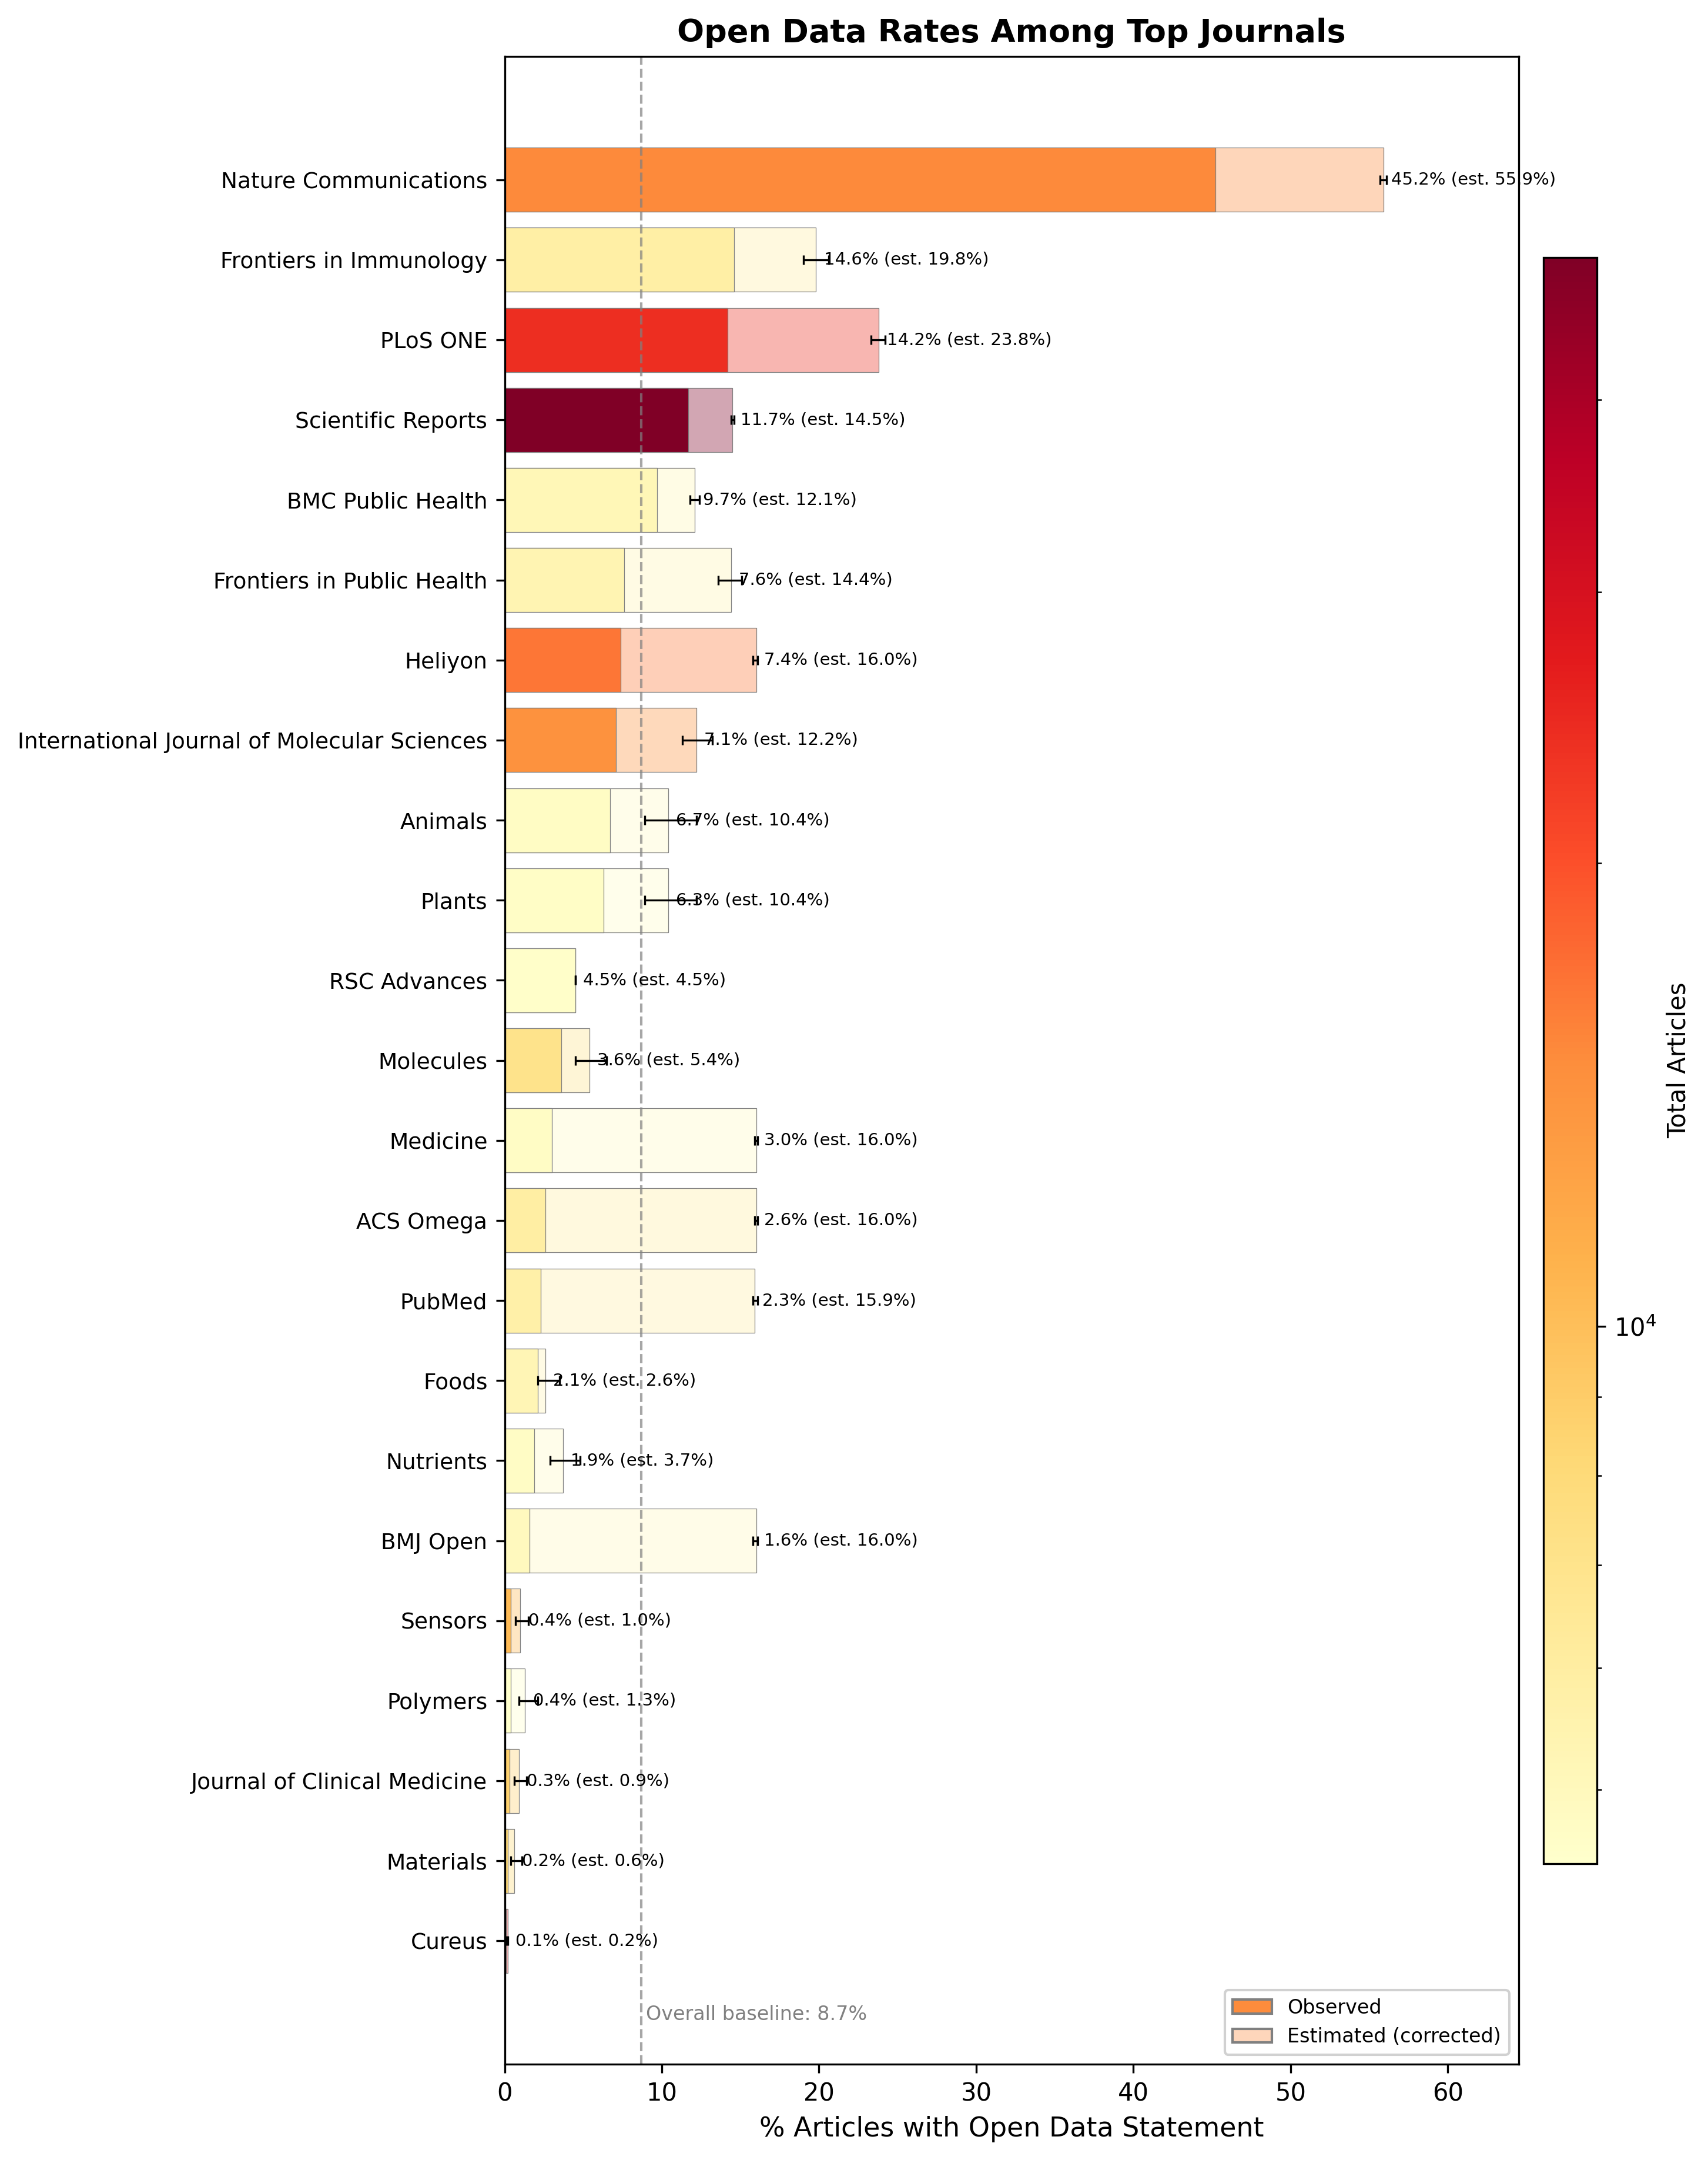
\includegraphics[width=\textwidth]{figures/journals_open_data_2024_2025.png}
\caption{Open data rates among top biomedical journals (2024--2025 research articles). Solid bars show the observed open data rate; lighter background bars show the estimated (corrected) rate after applying journal-level correction factors from head-to-head PDF vs.\ XML comparison. Error whiskers indicate 95\% Wilson score confidence intervals on the corrected estimate. Bar color encodes total article count on a log scale (yellow = fewer, red = more). Dashed line shows the overall baseline. Only journals exceeding the Weibull-derived survival article-count threshold are shown.}
\label{fig:journals}
\end{figure}

Journals in genomics and structural biology dominated the top ranks. Nature Structural \& Molecular Biology led with an observed rate of 86.1\% (130 of 151 articles) and an estimated rate of 91.7\% after correction for XML-only coverage. Microbial Genomics (84.8\%), Molecular \& Cellular Proteomics (81.6\%), Cell Genomics (80.2\%), and Genome Research (76.0\%) all exceeded 75\% observed. Nature Genetics achieved the highest estimated rate among all journals at 92.9\% (95\% CI: 91.5--93.7\%), reflecting the substantial uplift from PDF-based detection over its predominantly XML-only coverage. Genome Biology reached an estimated 89.3\% (95\% CI: 88.1--90.2\%).

A notable cluster of psychology and cognitive science journals also demonstrated high open data rates: the Journal of Cognition (72.8\%), Attention, Perception, \& Psychophysics (62.9\% observed, 68.2\% estimated), Psychological Research (62.2\%), Behavior Research Methods (59.8\%), and Communications Psychology (54.1\%). These rates likely reflect the growing open data culture in experimental psychology, driven by community norms and journal mandates that emerged in response to the replication crisis in that field.

Among the Nature portfolio, open data rates ranged from 86.1\% (Nature Structural \& Molecular Biology) to 45.2\% (Nature Communications), reflecting the diverse disciplinary scope of these journals and varying levels of field-specific data sharing norms. Nature Immunology (62.8\% observed, 79.1\% estimated), Nature Cell Biology (62.1\% observed, 76.3\% estimated), Nature Methods (59.0\% observed, 73.7\% estimated), and Nature Neuroscience (55.5\% observed, 69.8\% estimated) all showed substantial upward corrections, indicating that PDF-based detection captured data sharing statements missed by XML extraction in these journals.

High-volume journals provide insight into data sharing at scale. Scientific Data published \num{2421} articles in our window with a 65.6\% open data rate, consistent with its mission as a dedicated data journal. iScience (\num{3514} articles, 50.8\%), Communications Biology (\num{2503} articles, 47.2\% observed, 60.1\% estimated), and Nature Communications (\num{15129} articles, 45.2\% observed, 55.9\% estimated) demonstrate that moderately high rates are achievable even at very large publication volumes.

\subsection{Variation by Institution}

% TODO: Institution analysis not yet complete. This subsection will be populated
% when the institution pipeline (scripts/table_institutions.py) is finalized.
Institutional analysis is in progress and will be reported in a subsequent version of this manuscript. Preliminary results suggest that leading research universities and institutes achieve open data rates substantially above the baseline, consistent with patterns observed in the funder analysis (Table~\ref{tab:institutions}).

\subsection{Repository Adoption Patterns}

% TODO: Repository analysis not yet complete. This subsection will be populated
% when the repository pipeline is finalized.
Repository analysis is in progress and will be reported in a subsequent version of this manuscript. Preliminary examination of data sharing statements indicates that domain-specific repositories (e.g., GenBank, Protein Data Bank) and general-purpose repositories (e.g., Zenodo, Dryad, Figshare) both feature prominently (Table~\ref{tab:repositories}).

\subsection{Interactive Data Exploration}

\begin{quote}
\textbf{Interactive Dashboard:} Readers can explore these results dynamically through our web dashboard at \url{https://www.opensciencemetrics.org}, which provides real-time filtering and visualization across multiple dimensions including time periods, countries, and research domains.
\end{quote}


\section{Discussion}

\subsection{Key Findings}

Our analysis of approximately \num{326000} open access biomedical articles reveals that open data sharing is not uniformly distributed across the research ecosystem. The overall rate of 8.7\%---and even the 16.6\% funded-article baseline---falls far short of universal compliance with data sharing mandates. Yet the more than tenfold variation we observe, from single-digit percentages to above 90\%, demonstrates that high data sharing rates are achievable when appropriate incentives and requirements are in place.

The strongest predictor of high open data rates at both the funder and journal level appears to be the specificity and enforcement of data sharing policies combined with disciplinary norms that support sharing. Funders associated with data-intensive research (e.g., genomics, structural biology, environmental science) and those with strong institutional cultures of openness (e.g., EMBL, SciLifeLab, the Francis Crick Institute) achieve rates two to three times the funded-article baseline. Among journals, the pattern is even more striking: journals that require data deposit as a condition of publication (e.g., Nature Genetics, Genome Research) achieve rates above 75\%, while journals with weaker or absent data sharing requirements remain near or below the baseline.

\subsection{Comparison to Previous Work}

Our results extend and refine previous large-scale assessments of research transparency. Serghiou et al.\ documented the prevalence of multiple transparency indicators across biomedical publications using XML-based text mining~\cite{Serghiou2021-pl}. Our lower overall rate of 8.7\% likely reflects both the larger and more heterogeneous corpus (including articles from a broader range of journals) and the specificity of the oddpub v7.2.3 detection algorithm. Importantly, our PDF-based detection pipeline identifies approximately 52\% more open data statements than XML-based extraction on the same articles, demonstrating that previous XML-only estimates systematically undercount data sharing. This improvement is attributable to MinerU's ability to extract text from formatted data availability statements, supplementary sections, and other PDF elements not represented in PMC XML markup.

The correction factors we apply to account for XML-only coverage provide estimated rates that are consistently higher than observed rates, particularly for journals where a large fraction of articles lack PDF extraction. For example, Nature Genetics' observed rate of 70.5\% rises to an estimated 92.9\% after correction, reflecting the journal's strong data sharing culture that is partially masked by incomplete PDF coverage.

\textbf{Changes from preliminary results:} Some funders that featured prominently in our earlier presentation of these results no longer appear in the main figure. Most notably, the Howard Hughes Medical Institute (HHMI)---a private philanthropy that funds a relatively small number of elite investigators---achieved one of the highest per-article open data rates in the dataset (34.9\%, ranked 18th of 816 funders). However, HHMI's 748 funded articles in the 2024--2025 window fall well below the Weibull-derived figure threshold of $\geq$2,586 articles, and its 40,261 total OpenAlex works fall below the 100,000-work minimum applied to exclude small or niche funders. These thresholds, while necessary for focusing the figure on major world funders, systematically exclude high-performing private foundations with narrow funding portfolios. HHMI and similar funders (e.g., the Simons Foundation, the Chan Zuckerberg Initiative) remain visible in the full supplementary rankings. This pattern underscores that funder \emph{size} and funder \emph{effectiveness} at promoting open data are distinct dimensions that should be interpreted separately.

\subsection{Implications for Policy}

These results have several implications for research policy. First, they demonstrate that data sharing mandates \emph{work}: funders and journals with explicit, enforced requirements achieve markedly higher rates than those without. This finding supports continued investment in policy design and compliance monitoring. Second, the variation across funders with similar mandates suggests that policy stringency and enforcement mechanisms matter---not just the existence of a policy. Third, the disciplinary clustering we observe (genomics and psychology journals leading their respective tiers) indicates that community norms play an amplifying role beyond top-down mandates.

Our results also provide a benchmarking framework. Funders can compare their grantees' data sharing rates against peer organizations, journals can assess their position relative to comparable publications, and institutions can identify areas for targeted investment in data management infrastructure and training. The interactive dashboard at \url{https://www.opensciencemetrics.org} is designed to support exactly these comparisons.

\subsection{Limitations}

Several limitations should be noted. First, our corpus is restricted to open access articles available through PubMed Central; closed-access articles may exhibit different data sharing patterns, likely biased toward lower rates. Second, while oddpub v7.2.3 achieves high precision for detecting data sharing statements, it may miss non-standard phrasings or implicit data sharing (e.g., data available ``upon request''). Third, detecting a data sharing \emph{statement} is not equivalent to verifying that data are actually accessible and reusable; our rates should be interpreted as upper bounds on genuine data availability. Fourth, the correction factors assume that the head-to-head subset (articles with both PDF and XML) is representative of XML-only articles within each journal, which may not hold uniformly. Fifth, our two-year window (2024--2025) captures a snapshot of current practices but does not permit longitudinal analysis of trends over time.

\subsection{Future Directions}

Future work will expand the corpus to approximately \num{618000} articles as additional PDF processing completes, extend the temporal window through 2026, and complete the institution and repository analyses. Longitudinal analysis will enable assessment of whether specific policy changes (e.g., the 2023 NIH Data Management and Sharing Policy) are associated with measurable increases in data sharing rates. We also plan to incorporate repository-level analysis to characterize where shared data are being deposited and whether domain-specific or general-purpose repositories predominate across different research fields.

\subsection{Conclusion}

This study demonstrates that open data sharing in biomedicine varies more than tenfold across funders, journals, and disciplines. Major research funders achieve rates of 30--53\%, and leading journals reach estimated rates above 90\%, compared to an overall baseline of 8.7\%. These findings confirm that policy mandates and community norms can substantially increase data sharing, while also highlighting the considerable gap between current practice and universal compliance. Continued investment in scalable measurement tools, such as the pipeline and dashboard presented here, will be essential for monitoring progress toward a more open and reproducible research enterprise.


\section*{Data Availability}

Full results including all funder, journal, and institutional rankings are available as supplementary CSV files in the project repository. The interactive dashboard at \url{https://www.opensciencemetrics.org} provides dynamic exploration of all results. The oddpub detection pipeline and analysis code will be made available upon publication.
